% Title: gl2ps_renderer figure
% Creator: GL2PS 1.4.2, (C) 1999-2020 C. Geuzaine
% For: Octave
% CreationDate: Tue Oct 26 15:49:44 2021
\setlength{\unitlength}{1pt}
\begin{picture}(0,0)
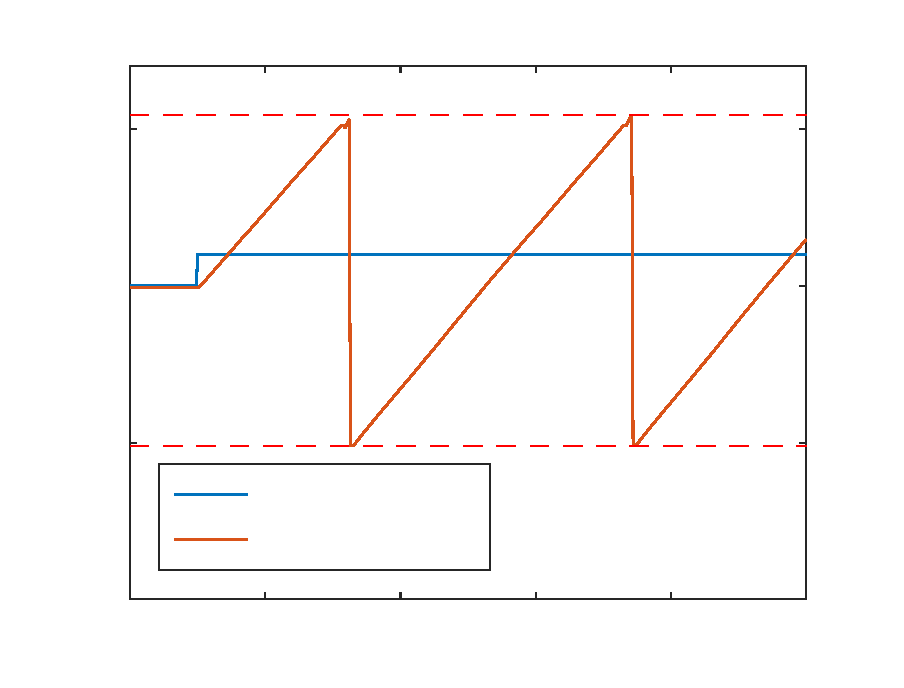
\includegraphics[scale=1]{motorDC2-inc}
\end{picture}%
\begin{picture}(418,314)(0,0)
\fontsize{10}{0}\selectfont\put(54.4343,27.0024){\makebox(0,0)[t]{\textcolor[rgb]{0.15,0.15,0.15}{{0}}}}
\fontsize{10}{0}\selectfont\put(119.337,27.0024){\makebox(0,0)[t]{\textcolor[rgb]{0.15,0.15,0.15}{{2}}}}
\fontsize{10}{0}\selectfont\put(184.239,27.0024){\makebox(0,0)[t]{\textcolor[rgb]{0.15,0.15,0.15}{{4}}}}
\fontsize{10}{0}\selectfont\put(249.142,27.0024){\makebox(0,0)[t]{\textcolor[rgb]{0.15,0.15,0.15}{{6}}}}
\fontsize{10}{0}\selectfont\put(314.044,27.0024){\makebox(0,0)[t]{\textcolor[rgb]{0.15,0.15,0.15}{{8}}}}
\fontsize{10}{0}\selectfont\put(378.946,27.0024){\makebox(0,0)[t]{\textcolor[rgb]{0.15,0.15,0.15}{{10}}}}
\fontsize{10}{0}\selectfont\put(49.4418,34.5008){\makebox(0,0)[r]{\textcolor[rgb]{0.15,0.15,0.15}{{-10}}}}
\fontsize{10}{0}\selectfont\put(49.4418,109.779){\makebox(0,0)[r]{\textcolor[rgb]{0.15,0.15,0.15}{{-5}}}}
\fontsize{10}{0}\selectfont\put(49.4418,185.057){\makebox(0,0)[r]{\textcolor[rgb]{0.15,0.15,0.15}{{0}}}}
\fontsize{10}{0}\selectfont\put(49.4418,260.335){\makebox(0,0)[r]{\textcolor[rgb]{0.15,0.15,0.15}{{5}}}}
\fontsize{11}{0}\selectfont\put(216.69,14.0024){\makebox(0,0)[t]{\textcolor[rgb]{0.15,0.15,0.15}{{Tempo (s)}}}}
\fontsize{11}{0}\selectfont\put(29.4418,162.474){\rotatebox{90}{\makebox(0,0)[b]{\textcolor[rgb]{0.15,0.15,0.15}{{Tensão (V)}}}}}
\fontsize{10}{0}\selectfont\put(249.142,94.7234){\makebox(0,0)[l]{\textcolor[rgb]{0,0,0}{{min: -5.0924 V $\implies 180^o$ }}}}
\fontsize{10}{0}\selectfont\put(249.142,275.391){\makebox(0,0)[l]{\textcolor[rgb]{0,0,0}{{max: 5.4437 V $\implies -180^o$ }}}}
\fontsize{9}{0}\selectfont\put(117.934,84.9481){\makebox(0,0)[l]{\textcolor[rgb]{0,0,0}{{Tensão de entrada}}}}
\fontsize{9}{0}\selectfont\put(117.934,63.0759){\makebox(0,0)[l]{\textcolor[rgb]{0,0,0}{{Tensão no potenciómetro}}}}
\end{picture}
